\section{HTTP/HTTPS}

%%%%%%%%%%%%%%%%%%%%%%%%%%%
%  Fonctionnement de HTTP %
%%%%%%%%%%%%%%%%%%%%%%%%%%%

\begin{frame}{Fonctionnement de HTTP}
    \begin{columns}
        \begin{column}{0.5\textwidth}
            \begin{block}{Protocole client-serveur}
                \begin{itemize}
                    \item{Client : requête HTTP}
                    \item{Serveur : envoi de la ressource}
                \end{itemize}
            \end{block}
        \end{column}

        \begin{column}{0.5\textwidth}
            \begin{exampleblock}{Navigateur web}
                \begin{itemize}
                    \item{Rend le processus transparent}
                    \item{Met en forme le html/css}
                \end{itemize}
            \end{exampleblock}
        \end{column}
    \end{columns}

    \hspace{40cm}

    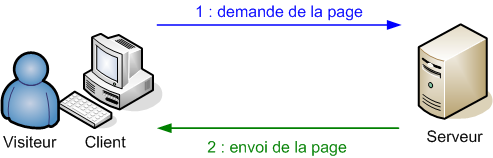
\includegraphics[width=\linewidth]{../medias/requete-http.png}
\end{frame}

%%%%%%%%%%%%%%%%%%%%%%%%%%%
%  Exemple de HTTP        %
%%%%%%%%%%%%%%%%%%%%%%%%%%%

\begin{frame}{Exemple d'une requête HTTP}
    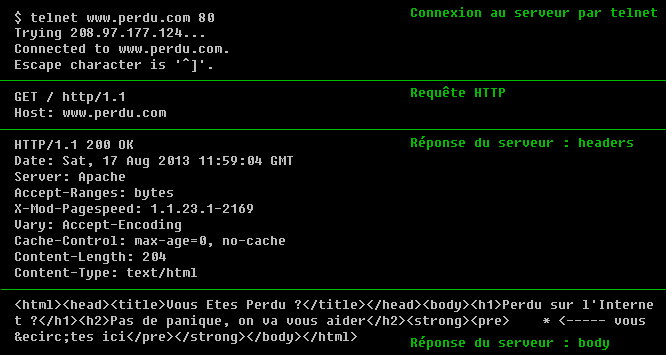
\includegraphics[width=\linewidth]{../medias/perdu.png}
    % Faire une petite démo en live (avec la même requête)
\end{frame}

%%%%%%%%%%%%%%%%%%%%%%%%%%%
%  HTTPS                  %
%%%%%%%%%%%%%%%%%%%%%%%%%%%

\begin{frame}{HTTPS : la version chiffrée de HTTP}
    
\includegraphics[width=\linewidth]{../medias/http-ssl.png}

    \hspace{10cm}

    % Dire à l'oral **qu'on ne touche pas à HTTP** et qu'on rajoute simplement le chiffrement par dessus
    \begin{columns}
        \begin{column}{0.5\textwidth}
            \begin{exampleblock}{Protocole SSL/TLS}
                \begin{itemize}
                    \item{Authentification du serveur}
                    \item{Confidentialité des données}
                    \item{Intégrité des données}
                \end{itemize}
            \end{exampleblock}
        \end{column}

        \begin{column}{0.5\textwidth}
            \begin{block}{Utilisé pour}
                \begin{itemize}
                    \item{Navigation web : HTTPS}
                    \item{Protocole mail : SMTPS}
                    \item{VPN : OpenVPN}
                \end{itemize}
            \end{block}
        \end{column}
    \end{columns}
    \hspace{20cm}

    {\Large \centerline{\alert{Limitation} : IP/port de destination toujours visible (pour routage)}}
\end{frame}


%%%%%%%%%%%%%%%%%%%%%%%%%%%
%  Certificats            %
%%%%%%%%%%%%%%%%%%%%%%%%%%%

\begin{frame}{Gestion des certificats}
    % Permet d'authentifier la communication \\
    % Sur internet, cela sert essentiellement à s'assurer de l'identité du serveur \\
    % Nécessité d'une authorité de certification (un tiers) \\
    \includegraphics[width=\linewidth]{../medias/autorite-certification.png}
\end{frame}

%%%%%%%%%%%%%%%%%%%%%%%%%%%
%  TLS                    %
%%%%%%%%%%%%%%%%%%%%%%%%%%%

\begin{frame}{Le protocole SSL/TLS}
    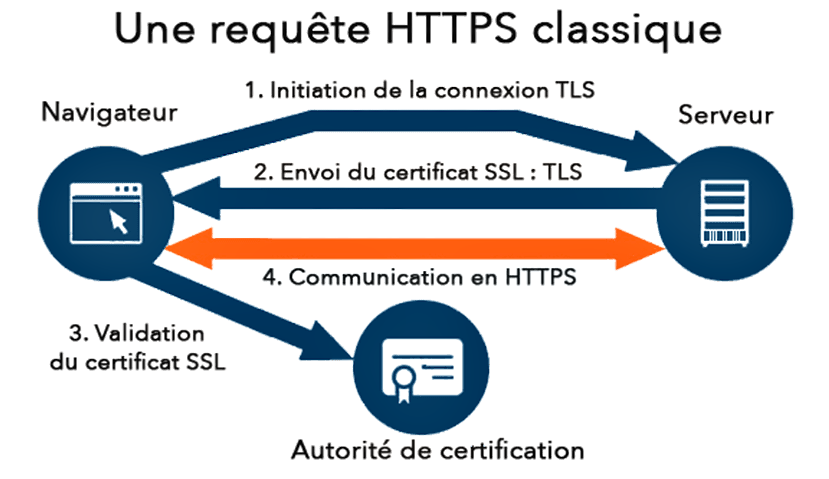
\includegraphics[width=\linewidth]{../medias/protocole-tls.png}
\end{frame}
